% !TeX root = ../main.tex

\chapter{绪论}

本章首先阐述了医学文本生成任务的研究背景和研究意义,并针对现有研究工作的现状进行介绍,从而引出本文的研究内容与创新点,最后介绍本文的组织结构。

\section{研究背景和意义}



%医学文本生成(Medical Text Generation)任务是一种基于自然语言处理(Natural language processing,NLP)技术面向电子病历(Electronic Health Record,EHR)、临床记录(Clinical Notes)等医学内容的特殊生成任务。近年来,其在EHR生成\cite{EHR_Generation}、临床记录生成\cite{CN_Generation}与生成式摘要\cite{Medical_Text_Generation_Summary_CN}等方面有着广泛的研究。医学文本生成任务是指使用自然语言生成技术,自动生成具有医学背景的自然语言文本,例如病历报告、症状描述、医疗建议等。这些文本通常需要准确地表达医学术语、疾病、症状、药物等复杂医学概念,以及具有一定的语法和逻辑性。医学文本生成任务可以用于辅助医学诊断和治疗,以及帮助医学人员生成病历、病情报告等文本。例如,医生可以通过输入患者的病情和症状信息,自动生成病历和诊断报告,减轻医生的工作负担,提高工作效率,避免错误和疏漏。此外,医学文本生成还可以用于帮助患者理解医学术语和治疗方案,提高患者的医疗健康素养。
%
%
%当前使用深度学习的NLP技术,在包括生成任务等各种下游任务中效果最显著的是 Transformer\cite{Attn_is_all_you_need}及其各种变体\cite{BERT, GPT2, GPT3}的语言模型(Language Model,LM),这类模型的参数量大,甚至达到了千亿的规模。虽然其在医学文本生成任务上的效果也优于其他模型,然而在医学文本生成任务中,满足这样规模的数据量是单个医疗机构难达到的。同时,由于患者的隐私需求以及各国法律法规(如欧盟的《通用数据保护条例》、中国的《关于印发国家健康医疗大数据标准、安全和服务管理办法(试行)的通知》)的限制,这种数据的收集与共享受到了进一步的限制。因此,如何在保护患者与医疗机构隐私的情况下训练文本生成模型并提供服务是一项挑战。由于上述的病历与记录内容包含关于患者大量的隐私内容,因此在训练生成模型与提供查询服务的过程中,一方面需要隐私数据在训练过程中对训练方不可见,另一方面在执行推断时需要防止模型直接泄露原始的文本内容。
%
%深度学习隐私保护的相关研究主要考虑两种不同的安全定义,一是防止从模型推导出一部分训练数据,例如判断数据是否在训练集中,或根据模型参数重建部分训练集等,通常采用的方法是差分隐私技术.第二种是防止学习算法的运行者访问数据或模型,通常采用安全多方计算或同态加密算法来实现。
%
%
%在训练阶段中,隐私数据面临着直接的威胁。由于“数据孤岛”现象,多个数据持有者有充分的动机协同训练大型LM(激励公平不在安全性的讨论范围内)。已有的工作主要使用联邦学习(Federated learning,FL)的方式\cite{FL_ZS},使得各数据持有者可以充分利用各方数据进行协同训练。而在NLP任务中,特别地,在医学文本生成任务的情况下,各数据持有者(医院)的EHR文本类型的诊断数据包含该数据持有者的一些独特特征(如医生的写作风格,数据持有者对原始数据的转换整理方式),即各数据持有者的数据非独立同分布。在这种情况下,FL处理方式的精度较低\cite{CC_FL, FL_Medical_Relation_Extraction, FL_CMF}。此外,研究\cite{grad_leak_privacy}表明攻击者可以利用模型任何层的输出以及梯度信息重建训练样本。因此,探索如何保障数据在训练阶段的隐私性有着重要价值。
%
%在推断阶段中,模型可能会在“不经意间”泄露训练数据。研究工作\cite{Extrac_Train_Data_From_LM, RealToxicityPrompts, Counterfactual, LMPPMean, mireshghallah2022memorization}证明了LM具有记忆性,特别是在给定特定的前缀(Prefix)时,LM甚至可以逐字逐句地生成出原始的训练样本。攻击者可以大量枚举多种前缀来对LM执行训练数据提取攻击与成员推断攻击。在医学文本生成的场景下,前缀的搜索空间更小,更容易定制,如“医生给我开的”、“现在只是稍有点咳嗽”等前缀是很容易联想到的,攻击者的攻击效率与成功率也会更高。因此,如何防范针对医学文本生成的LM在推断时泄露隐私数据成为一项重要的问题。
%
%此外,当前开源的中文预训练模型资源较少。另一方面,由于现有的常见开源预训练模型\cite{BERT, GPT2}的训练语料中英文占比在80\%以上,而不同语言之间的词向量(Word Embedding)与模型参数之间差别较大,迁移学习的效果不理想\cite{Transfer_Learning_4LM_Generation, Multi_NMT},故直接使用这些预训练模型做中文场景下任务的微调效果不好。因此,要想验证医学文本生成任务的LM记忆问题还要面向医学文本数据进行微调训练。

%此外,研究\cite{grad_leak_privacy}表明攻击者可以利用模型任何层的输出和梯度信息重建训练样本。

%在训练阶段,隐私数据面临直接威胁。由于法律法规限制多个拥有患者隐私文本数据的医疗机构之间的数据收集与共享,现有的研究主要采用两种隐私保护的方式来缓解数据稀缺的问题:联邦学习(Federated Learning,FL)方式与集中式学习方式。联邦学习(Federated Learning,FL)方式\cite{FL_ZS},使各数据持有者能够充分利用各方数据进行协同训练。然而,在NLP任务中,特别是医学文本生成任务中,各数据持有者(如医院)的EHR文本类型诊断数据包含数据持有者的一些独特特征(如医生写作风格和数据持有者对原始数据的转换整理方式),导致各数据持有者的数据非独立同分布。在这种情况下,FL的处理精度较低\cite{CC_FL, FL_Medical_Relation_Extraction, FL_CMF}。此外,研究\cite{grad_leak_privacy}表明攻击者可以利用模型任何层的输出和梯度信息重建训练样本。因此,探究如何保障数据在训练阶段的隐私性具有重要意义。

%综上所述,本研究将针对医学文本生成任务中的隐私保护问题展开探讨,分析训练阶段和推断阶段的隐私泄露风险,以及如何在保护隐私的前提下实现高效的医学文本生成。我们将关注差分隐私、安全多方计算和同态加密等技术在医学文本生成任务中的应用,以期为医疗领域提供一种安全、高效且实用的文本生成解决方案。

%目前,基于深度学习的NLP技术在各种下游任务中,尤其是生成任务中,取得了显著的效果


本节首先介绍医学文本生成任务的基本概念,并对其研究背景和研究意义进行详细说明。

\subsection{研究背景}

医学文本生成(Medical Text Generation)任务是一种针对电子病历(Electronic Health Record,EHR)和临床记录(Clinical Notes)等医学内容的自然语言处理(Natural Language Processing,NLP)技术。近年来,医学文本生成在电子病历生成\cite{EHR_Generation}、临床记录生成\cite{CN_Generation}以及生成式摘要\cite{Medical_Text_Generation_Summary_CN}等领域得到了广泛应用。医学文本生成任务旨在利用自然语言生成技术自动生成具有医学背景的自然语言文本,如病历报告、症状描述和医疗建议等。这些文本需要准确表达医学术语、疾病、症状、药物等复杂医学概念,同时具备一定的语法和逻辑性。医学文本生成任务可以辅助医学诊断和治疗,帮助医务人员生成病历和病情报告,提高工作效率和减轻工作负担,同时避免错误和疏漏。此外,医学文本生成还有助于患者理解医学术语和治疗方案,提高患者的医疗健康素养。

Transformer\cite{Attn_is_all_you_need}及其各种变体\cite{BERT, GPT2, GPT3}的语言模型(Language Model,LM)在医学文本生成任务上的表现优于其他模型。然而,这类模型通常具有庞大的参数量,达到千亿规模。在医学文本生成任务中,考虑到病历和记录中包含大量患者隐私信息,满足如此规模的数据量对单个医疗机构来说是难以实现的。同时,受到患者隐私需求及各国法律法规\footnote{欧盟的《通用数据保护条例》}\footnote{中国的《关于印发国家健康医疗大数据标准、安全和服务管理办法(试行)的通知》}的限制,数据的收集和共享面临更大的挑战。因此,在保护患者和医疗机构隐私的前提下,训练文本生成模型并提供服务成为了一项重要的挑战。此外,语言模型面临着记忆问题,即语言模型容易记住训练数据中出现的特定内容,并会在推断阶段输出训练数据的部分内容。在医学文本生成任务下,语言模型的使用可能会导致患者隐私泄露的风险。因此,解决语言模型记忆问题亦成为一项紧迫任务。

基于语言模型的医学文本生成任务的隐私保护研究主要关注两种安全问题:一方面是是防止执行学习训练与推断算法的计算方访问数据或模型,通常采用安全多方计算(Multi-party Secure Computation, MPC)或同态加密算法实现;另一方面是是防止模型使用者从模型的推断结果恢复出部分训练数据,如根据模型参数或模型推断结果判断特定数据是否在训练集中或重建部分训练集,通常采用差分隐私(Differential Privacy,DP)技术。

在训练阶段,隐私数据面临直接威胁。由于法律法规限制多个拥有患者隐私文本数据的医疗机构之间的数据收集与共享,现有的研究主要针对两种训练方式,即联邦学习\cite{FL_ZS}(Federated Learning,FL)方式与集中式学习方式。为保护训练数据以及模型参数的隐私,研究者将差分隐私\cite{DP}、多方安全计算\cite{cramer2015secure}、同态加密\cite{acar2018survey}与可信执行环境\cite{sabt2015trusted}(Trusted Execution Environment,TEE)等隐私保护技术与联邦学习或者集中式学习相结合。这两种学习方式均可使各数据持有者充分利用各方数据进行协同训练。然而,在NLP任务中,特别是医学文本生成任务中,各数据持有者(医疗机构)的EHR文本类型数据通常包含该数据持有者的一些独特特征(如医生写作风格和数据持有者对原始数据的转换整理方式),导致各数据持有者的数据非独立同分布。在这种情况下,联邦学习方式的训练精度较低\cite{CC_FL, FL_Medical_Relation_Extraction, FL_CMF}。相较于联邦学习方式,集中学习方式训练的模型精度较高,但同时面临的隐私风险也会更高,与此同时,当前针对集中式学习的隐私保护研究面临着安全假设弱的问题。因此,在医学文本生成任务的训练阶段,探究如何保护隐私训练数据以及模型参数具有重要意义。

在推断阶段,语言模型可能会在无意中泄露训练数据。当前多项研究\cite{Extrac_Train_Data_From_LM, RealToxicityPrompts, Counterfactual, LMPPMean}证实了语言模型具有记忆性。记忆性是指模型容易记住训练数据中出现的特定内容,即语言模型可能会推断阶段输出训练数据的部分内容。在给定特定前缀(Prefix)时,语言模型甚至可以逐字逐句地生成原始训练样本。攻击者可以大量枚举多种前缀,对语言模型执行模型反演攻击来恢复训练数据中的隐私信息。在医学文本生成场景下,前缀的搜索空间更小,更容易定制,如“医生给我开的”和“现在只是稍有点咳嗽”等前缀容易联想到,攻击者的攻击效率和成功率也会比其他场景更高。因此,如何在医学文本生成的语言模型进行推断时有效防止隐私数据泄露,成为当前亟待解决的重要问题。


%此外,目前开源的中文预训练模型资源较少。另一方面,由于现有常见开源预训练模型\cite{BERT, GPT2}的训练语料中英文占比在80\%以上,而不同语言之间的词向量(Word Embedding)和模型参数差异较大,迁移学习效果不理想\cite{Transfer_Learning_4LM_Generation, Multi_NMT}。因此,直接使用这些预训练模型在中文场景下进行任务微调效果不佳。为验证医学文本生成任务的LM记忆问题,还需针对医学文本数据进行微调训练。

此外,目前开源的中文预训练模型资源有限。现有的预训练模型\cite{BERT, GPT2}的训练语料中英文占比在80\%以上,迁移学习效果不理想\cite{Transfer_Learning_4LM_Generation, Multi_NMT}。为验证医学文本生成任务的语言模型记忆问题,还需针对医学文本数据进行微调训练。

\subsection{研究意义}

%当前已有的相关研究面临着很多问题。首先,针对训练阶段来说,已有的工作主要使用FL的方式。一方面,这些工作都假设集中聚合模型梯度的计算方是半诚实的,这种假设安全性较弱。另一方面,在FL的方式下训练的模型性能差于使用全部数据进行集中训练的方式。其次,针对推断阶段来说,已有的工作是使用差分隐私(Differential Privacy,DP)技术\cite{DP}来保护隐私数据的。然而,对所有数据进行DP处理会导致模型精度低\cite{DP_Text_Analytics},单独对隐私部分处理的工作的筛选机制不现实。为了解决上述问题,本文的主要意义如下:
%
%\begin{itemize}
%	\item [$\cdot$]
%	本文分别为医学文本生成任务在训练与推断两种场景下的攻击进行了详细的分类,并分析其攻击手段的隐私威胁程度。在训练阶段,本章考虑攻击者试图推断隐私数据并且破坏训练协议的场景。在推断阶段,本章考虑攻击者试图通过执行输入和标签重构攻击来恢复训练隐私数据的场景。这部分的研究为后续两阶段的隐私保护工作研究提供了铺垫。
%	\item [$\cdot$]
%	本文通过集中化训练的方式,使用可信执行环境(Trusted Execution Environment,TEE)并设计了一套面向建模医学文本生成模型的多方安全计算协议来提升安全假设。这为训练医学文本生成模型提供了一种隐私保护的方法。
%	\item [$\cdot$]
%	本文通过引入一个新颖的差分隐私定义,并针对训练与推断阶段分别设计了一个符合该差分隐私定义的算法,以保护模型的训练隐私数据不会被攻击者获取。这为缓解LM的记忆问题提供了新的措施,同时避免牺牲过多的精度。
%\end{itemize}

%一方面,这些研究都假设集中聚合模型梯度的计算方是半诚实的,这种假设的安全性较弱。

当前已有的相关研究面临诸多挑战。首先,在训练阶段,现有采用联邦学习的研究,由于医学文本数据的非独立同分布性质导致训练精度较低\cite{CC_FL, FL_Medical_Relation_Extraction, FL_CMF}。而使用集中式学习方式的工作面临的隐私风险更高,目前针对集中式学习的隐私保护研究面临着安全假设弱的问题\cite{SecureNLP, SecureNN, secgnn, Cryptflow}。其次,在推断阶段,现有研究采用差分隐私(Differential Privacy,DP)技术\cite{DP}来保护隐私数据。然而,对所有数据进行DP处理会导致模型精度降低\cite{DP_Text_Analytics}。针对上述问题,本研究的主要意义如下:

%然而,在NLP任务中,特别是医学文本生成任务中,各数据持有者(医疗机构)的EHR文本类型数据通常包含该数据持有者的一些独特特征(如医生写作风格和数据持有者对原始数据的转换整理方式),导致各数据持有者的数据非独立同分布。在这种情况下,联邦学习方式的训练精度较低\cite{CC_FL, FL_Medical_Relation_Extraction, FL_CMF}。而集中式学习方式面临的隐私风险更高,目前针对集中式学习的隐私保护研究面临着安全假设弱的问题。

%因此,本文针对恶意的参与者参与的训练阶段,通过引入多方安全计算(Multi-party Secure Computation, MPC)与可信硬件 Intel SGX,并设计了一个安全的LM训练协议来保护训练数据以及模型的安全;同时为有效缓解语言模型的记忆问题,防止恶意攻击者通过模型反演攻击来获取训练隐私数据,本文基于差分隐私,有效的缓解了语言模型的记忆问题。


\begin{itemize}
	\item [$\cdot$]
	本文针对医学文本生成任务在训练和推断两个阶段的攻击场景进行分类,并分析了各类攻击手段对隐私安全的威胁程度。在训练阶段,考虑攻击者试图推断隐私数据并破坏训练协议的场景;在推断阶段,考虑攻击者试图恢复训练中的隐私数据的场景。这一部分研究为后续隐私保护策略的设计奠定了基础。
	\item [$\cdot$]
	本文借助可信硬件Intel SGX设计了一套针对医学文本生成模型的多方安全计算协议,以提升安全性假设。该协议在面对恶意攻击者的情况下仍能保证安全性,为训练医学文本生成模型提供了一种创新的隐私保护方法。
	\item [$\cdot$]
	本文基于差分隐私技术,针对训练阶段提出了一种差分隐私优化器;针对推断阶段设计了一个差分隐私解码算法。通过上述两种方法缓解语言模型的记忆问题,防止模型的训练隐私数据被攻击者获取,同时避免牺牲过多的精度。
\end{itemize}

本研究旨在提供一种针对医学文本生成任务的隐私保护方法,通过对训练阶段和推断阶段的隐私保护技术的探讨与改进,为后续研究和实际应用提供了重要的参考和借鉴。本文针对训练阶段中存在恶意参与者的问题,引入多方安全计算与可信硬件 Intel SGX,并设计了一个安全的语言模型训练协议来保护训练数据以及模型的安全;同时为有效缓解语言模型的记忆问题,防止恶意攻击者通过模型反演攻击来获取训练隐私数据,本文引入差分隐私,有效的缓解了语言模型的记忆问题。

本研究的深入分析和实践将有助于提高医学文本生成模型的隐私保护水平,降低数据泄露风险,保障患者隐私,同时不影响模型性能。此外,本研究的成果对于其他涉及敏感数据的自然语言处理任务也具有一定的参考价值,有助于推动隐私保护技术在自然语言处理领域的进一步发展。

%%(1)首先,我们根据阶段与攻击形式的不同,本文分别对医学文本生成任务在训练与推断两种场景下执行相应的攻击。在训练阶段,本章考虑攻击者试图推断隐私数据并且破坏训练协议的场景。在推断阶段,本章考虑攻击者试图通过执行输入和标签重构攻击来恢复训练隐私数据的场景。最后通过实验结果说明其攻击效果并分析对应的隐私保护手段。
%
%(1)首先,目前还没有在中文LM上执行攻击的研究,更不用说针对医学文本生成任务的攻击。本文根据阶段与攻击形式的不同,本文分别对医学文本生成任务在训练与推断两种场景下执行相应的攻击。在训练阶段,本章考虑攻击者试图推断隐私数据并且破坏训练协议的场景。在推断阶段,本章考虑攻击者试图通过执行输入和标签重构攻击来恢复训练隐私数据的场景。最后通过实验结果说明其攻击效果并分析对应的隐私保护手段。
%
%(2)其次,为了解决现有工作中安全假设较弱的问题,本文使用可信执行环境(Trusted Execution Environment,TEE)提升安全假设,即使是恶意的计算方也不能偏离协议;通过集中化训练的方式,使用多方安全计算(Multi-party Secure Computation,MPC)协议保证执行过程的机密性,同时拓展MPC协议以支持Transformer结构的模型。
%
%(3)最后,为了使攻击者不会通过模型恢复出参与训练的隐私数据,本文提出了一个新颖的选择差分隐私策略。通过对文本的隐私性进行分类,并针对隐私部分使用DP处理,实现了在不牺牲过多精度的同时保护隐私数据。


\section{研究现状}

本节首先介绍语言模型的记忆问题及其带来的隐私风险,随后介绍基于多方安全计算的医学文本生成任务的研究状况,最后分析基于差分隐私的医学文本生成任务的研究进展。

\subsection{语言模型的记忆问题}

随着深度学习技术的快速发展,大型语言模型在自然语言处理领域取得了重要突破。例如,GPT\cite{GPT2, GPT3, GPT4}系列和BERT\cite{BERT}模型已在多个任务上实现了超过人类的性能,近期的ChatGPT以及GPT4\cite{GPT4}的表现效果更为惊人,似乎有着与人类相同的表达能力。然而,随着模型规模的扩大,其在学习过程中对训练数据的记忆问题引起了人们的关注。具体而言,LM的记忆问题是指LM在输出时更倾向于输入在训练样本中出现过的内容,在一定条件下甚至可以逐字逐句地生成完整的训练语句。研究表明,这些LM可能会在生成结果中泄露训练数据中的敏感信息。

例如,Gehman等人\cite{RealToxicityPrompts}调查了预训练LM在生成带有种族主义、性别歧视或其他有害语言方面存在的问题。作者调查了预训练语言模型在受到特定提示时生成有害语言的程度,并研究了可控文本生成算法在防止生成这种有害语言方面的效果。为了找出这种持续的有害退化的潜在原因,作者对用于预训练多个语言模型(包括GPT-2)的两个网络文本语料库进行了分析,并发现了大量的攻击性、事实不可靠和其他有害内容。这些发现证明了语言模型具有记忆性。Nicholas等人\cite{Extrac_Train_Data_From_LM}研究了私有数据集上训练的大型语言模型可能存在的训练数据提取攻击。攻击者可以通过查询语言模型来恢复单个训练样本。作者在GPT-2模型上演示了这种攻击,该模型是基于互联网公开的数据进行训练的。他们成功地从模型的训练数据中提取了数百个逐字文本序列。尽管上述序列中的每一个只出现在训练数据的一个文档中,但攻击仍然可行。作者全面评估了提取攻击,以了解导致其成功的因素。这些发现表明,更大的模型比较小的模型更易受到攻击。Zhang等人\cite{Counterfactual}探讨了现代神经语言模型在训练过程中可能会记忆敏感信息的问题。作者提出了反事实记忆的概念,它描述了在省略训练过程中的某个特定文档的情况下,模型预测的变化。通过在标准文本数据集中识别和研究反事实记忆的训练样本,作者进一步估计了每个训练样本对验证集和生成文本的影响。Brown等人\cite{LMPPMean}探讨了自然语言隐私问题的广泛性。作者指出,语言模型往往会记忆训练集中存在的短语,而攻击者可以利用这种倾向来提取训练数据,违反隐私期望。作者讨论了常见数据保护技术(数据清理和差分隐私)所做的狭隘假设与自然语言和隐私作为社会规范的广泛性之间不匹配的问题,认为现有的保护方法不能为语言模型提供通用且有意义的隐私保护。Mireshghallah等人\cite{mireshghallah2022memorization}研究了大型语言模型微调过程中不同微调方法(对整个模型、模型头部和适配器进行微调)的记忆风险,并使用成员推断和提取攻击进行实验。作者的研究表明微调模型头部的风险最高,而微调较小的适配器则不容易受到已知提取攻击的影响。这对于“预训练和微调”范式的应用具有重要意义。

为了解决语言模型的记忆问题,研究者已经开始探索在训练过程中防止模型记忆敏感信息的方法。其中一种方法是改进模型结构,例如引入注意力机制或使用门控循环单元等,这些改进有助于提高模型处理长序列的能力,从而减少对敏感信息的依赖。另一种方法是优化训练过程,例如使用数据增强、对抗训练和知识蒸馏等技术,这些方法可以提高模型的泛化能力,缓解模型对训练数据的过拟合问题。

%因此,语言模型的记忆问题存在挑战。因此,本文在第三章总结概述了医学文本生成任务训练与推断阶段面临的攻击,并在第五章基于差分隐私设计了隐私保护方法来缓解语言模型的记忆问题。

因此,语言模型的记忆问题给隐私保护带来了挑战。鉴于此,本文在第3章详细概述了医学文本生成任务在训练和推断阶段所面临的各种攻击,并在第5章基于差分隐私原理设计了隐私保护方法,以缓解语言模型的记忆问题。

%如何在保证模型性能的同时有效防止敏感信息泄露,以及如何在实际应用中选择合适的隐私保护技术等问题,仍需进一步研究。

%然而RNN的表达能力有限,要取得高表达能力的效果,需要使用基于Transformer结构的语言模型。因此,本文在第三章

\subsection{基于多方安全计算的医学文本生成任务}

本部分首先介绍基于多方安全计算的深度学习隐私保护技术,然后阐述目前用于医学NLP任务上的多方安全计算的相关工作。

基于多方安全计算的隐私保护深度学习旨在模拟存在可信第三方的计算过程,使得计算过程不会泄露隐私信息,但是其无法为保护模型参数与推断结果提供隐私保护。最经典的隐私保护机器学习框架是由Mohassel和Zhang设计的SecureML\cite{secureml}。该方案是基于两个服务器Client/Server的使用秘密共享的外包计算模型。其中,服务器从多个客户端接收以秘密份额形式的数据,并基于SPDZ框架\cite{spd}与混淆电路对秘密份额数据进行隐私训练和预测。与SPDZ框架类似,为保证训练与推断的及时响应,SecureML在离线阶段执行复杂运算,从而使得在线阶段处理效率更高。基于Wu等人\cite{wu2018training}通过量化方法减少隐私保护训练阶段中的精度损失,Agrawal等\cite{agrawal2019quotient}在半诚实攻击者的场景下,设计了QUOTIENT协议。该协议使用加法秘密共享机制和Yao混淆电路,实现了随机梯度下降算法和自适应梯度下降算法这两种深度学习模型的训练算法。董业等人\cite{FLSSGS}使用秘密共享机制和Top-K梯度筛选方法来保护训练阶段中梯度信息的隐私,并且能够验证服务器聚合结果的有效性。Patra等人\cite{patra2021aby2}基于布尔域、算数域和Yao混淆电路域上的混合秘密共享机制设计了ABY 2.0,其实现了半诚实攻击者场景下的线性回归和卷积网络的训练。进一步地,Mohassel\cite{mohassel2018aby3}等人提出的ABY3在ABY1\cite{demmler2015aby}的框架上将原算法进行了扩展,使用三方计算场景进行训练和评估。其可以在布尔域、算数域和Yao混淆电路域之间高效地切换,并可以在半诚实攻击者场景下用在训练线性回归、逻辑回归和神经网络模型上。Wagh等人\cite{SecureNN}的算法也基于三方服务器,但其第三方服务器并不与秘密份额交互,其仅用于提供运算辅助。Rachuri等人\cite{chaudhari2019trident}基于结合ABY3和第三方服务器,首次实现了在恶意攻击者场景下的安全训练。

目前基于MPC用于NLP领域的主要工作是Feng等人\cite{SecureNLP}提出的隐私保护系统SecureNLP,其重点针对用于神经机器翻译的基于循环神经网络(Recurrent Neural Network,RNN)的序列到序列注意力模型。具体来说,针对Sigmoid和tanh等非线性函数,作者使用MPC设计了两个高效的分布式协议,用于在SecureNLP中执行各自的任务。作者还证明了这两个协议(即隐私保护的长短时记忆网络PrivLSTM和隐私保护的序列到序列转换PrivSEQ2SEQ)在半诚实攻击者模型下是安全的,即任何诚实但好奇的攻击者不能从他们从其他方接收到的消息中了解到任何其他信息。

%然而RNN的表达能力有限,要取得高表达能力的效果,需要使用基于Transformer结构的语言模型。因此,本文在第四章基于多方安全计算设计了一套用于Transformer结构模型的协议。

然而,RNN的表达能力存在局限性,要实现更高的表达能力,需要采用基于Transformer结构的语言模型。因此,在本文的第4章中,我们基于多方安全计算设计了一套适用于Transformer结构模型的协议,以满足更高表达能力的需求。

\subsection{基于差分隐私的医学文本生成任务}

与上述结构相同,本部分首先介绍基于差分隐私的机器学习隐私保护技术,然后阐述目前用于医学NLP任务上的差分隐私的相关工作。

差分隐私技术通过在数据输入、算法迭代或算法输出中添加随机噪声来抵抗隶属关系猜测攻击。例如Dwork等人\cite{DP}进行特征分解之前,在协方差矩阵中加入对称高斯噪声矩阵,使得输出结果是一个差分隐私的投影矩阵。Hardt和Price\cite{hardt2014noisy}则在算法每次迭代中添加高斯噪声,而协方差矩阵保持无扰动状态,实现一个差分隐私的主成分分析。Abadi\cite{abadi2016deep}等人则是在随机梯度下降算法的迭代中引入高斯噪声,实现了深度神经网络学习的数据隐私。Wu等人\cite{wu2018training}通过对输出数据添加噪声扰动,实现了具有隐私保护的线性回归和决策向量机等二分类模型。以上工作均为数据持有者独立训练采用的隐私保护方法。为实现多源数据集的隐私聚合训练,Papernot\cite{papernot2016semi}等人提出,首先利用互相独立的数据集学习教师模型,然后使用这些教师模型对公共数据进行带噪声的预测,最后将预测结果迁移到学生模型的构建。该方法中隐私损失取决于学生模型训练期间向教师模型提出的查询次数,与最终投入实用的学生模型的查询次数无关。梁文娟等人面向数据流Top-K频繁模式挖掘,基于差分隐私,设计了动态发布过程的数据隐私保护方案。史鼎元\cite{CDFL}等人则基于略图数据结构和差分隐私技术,解决排序学习中的交叉特征生成和缺失标签处理问题。

目前基于DP用于NLP领域的工作有很多。Bombari等人\cite{bombari2022towards}探讨了训练数据集中实体之间的关系被记忆,即可能在使用训练好的模型进行问答时产生隐私问题的问题。作者提出了关系记忆的概念,并规范化了关系隐私的概念。同时,作者还提出了差分关系隐私的潜在定义,用于描述和计算模型中RM的量的界限。Zhao等人\cite{zhao2022provably}提出了一种名为机密去重训练的保密调整训练方法,用于训练语言生成模型时保护隐私信息。该方法借鉴了差分隐私的思想,通过随机化部分训练过程来防止意外记忆,并证明了大致正确的筛选策略可以增强保密性保证。实验结果表明,机密去重训练方法在保持强大保密性的同时,能够获得几乎相同的困惑度。Wu等人\cite{DPSSGD}提出了自适应差分隐私框架来保护语言模型不泄露隐私信息,避免了传统差分隐私在所有数据点上的不加区分保护所带来的实用性问题。与之前需要先验隐私信息的方法不同,自适应差分隐私基于语言模型估算文本项含有隐私信息的概率,并根据该概率调整注入差分隐私噪声的程度。本文还提出了一种新的Adam算法来实现这一目标。实验结果表明,自适应差分隐私框架能够有效地提高差分隐私语言模型的保护能力,防止Canary攻击。Shi等人\cite{selectivedp}提出了部分差分隐私,以提供对敏感数据的严格隐私保护,以提高模型效用。作者开发了一个相应的隐私机制DPSGD优化器,用于基于RNN的语言模型。


%总的来说,基于差分隐私的医学文本生成任务的相关研究工作主要关注如何在保护隐私的前提下提高模型的性能和效率,以及如何利用新的隐私保护概念和算法来解决现有算法的局限性。因此,本文在第五章基于差分隐私针对训练与推断阶段分别设计了训练隐私优化器以及解码算法。

总体而言,基于差分隐私的医学文本生成任务的相关研究主要关注在保护隐私的前提下如何提升模型的性能和效率,以及如何运用新的隐私保护理念和算法来应对现有方法的局限性。因此,本文第5章针对训练和推断阶段分别设计了基于差分隐私的训练隐私优化器以及解码算法,以满足这些需求。

%其中,一些论文提出了新的隐私保护概念和机制,如部分差分隐私和自适应差分隐私,并开展了相关的实验来验证这些方法的有效性和实用性。此外,还有一些论文研究了如何对模型训练的不同阶段进行隐私保护,以及如何选择不同的模型微调方法来降低隐私泄露风险。

\section{研究内容与创新点}

本节对本文的研究内容进行介绍,并总结创新之处。

\subsection{研究内容}

医学文本生成任务相对于普通文本生成任务而言,对表达能力和逻辑性有更高的要求,因此普通文本通用的RNN模型不适用于医学文本任务。本文选择参数量大、表达能力强的Transformer模型解决上述问题。同时,本文也考虑了Transformer模型带来的记忆问题。综上所述,本文首先分析基于Transformer模型的医学文本生成任务在训练和推断阶段分别存在的隐私问题,再分别针对训练和推断阶段存在的隐私风险提出相应的隐私保护方案。

本文的主要研究内容总体框架如图\ref{Three_Chap_Structure}所示。

\begin{figure}[h]
	\centering
	%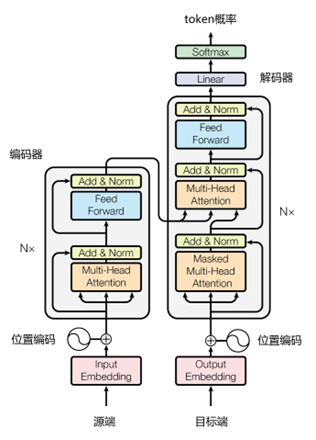
\includegraphics[width=1\textwidth]{figures/Transformer_Structure.png}
	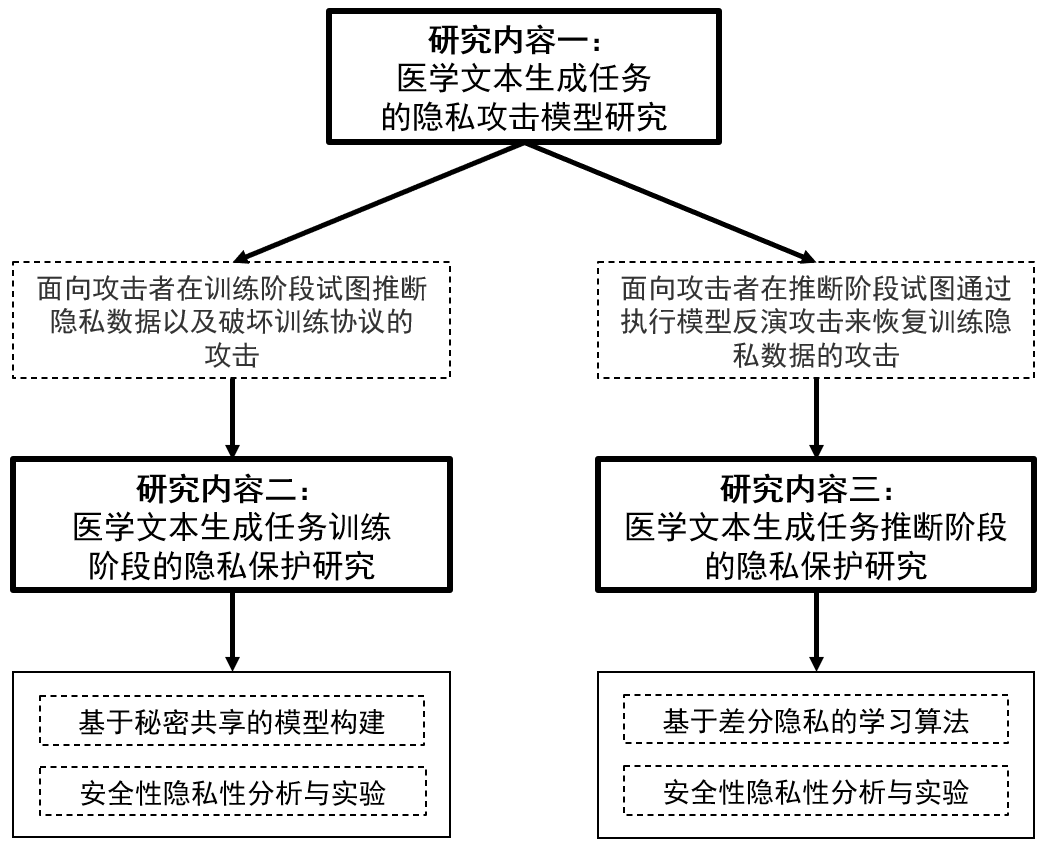
\includegraphics[width=0.85\linewidth]{figures/Three_Chap_Structure.png}
	\caption{本文的研究点以及主要研究内容}
	\label{Three_Chap_Structure}
\end{figure}

(1)医学文本生成任务的隐私攻击模型研究

本部分主要关注医学文本生成任务在训练和推断阶段的隐私泄露风险,以证实后续提出的隐私保护方法的重要性。首先,本研究内容从语言模型的生成过程出发,详细阐述了如何为自然语言文本建模并生成后续文本,为后续分析医学文本生成模型的训练与推断阶段的执行过程奠定基础。接着,本研究内容分析了语言模型的记忆问题,并针对公开的预训练模型实施模型反演攻击。同时,本研究内容还提出了一些改进的攻击策略,以提高攻击成功率。此外,本研究内容探讨了攻击者在医学文本生成任务的训练阶段可能采用的推断隐私数据和破坏训练协议的攻击手段。最后,从医学文本生成任务推断阶段的攻击以及上述改进攻击手段出发,通过对医学文本数据下训练的语言模型实施攻击,分析攻击效果,展示了语言模型记忆问题带来的隐私挑战。


(2)医学文本生成任务训练阶段的隐私保护研究


本部分主要关注医疗文本生成任务训练阶段的隐私保护问题。首先,本研究内容明确了系统模型和威胁模型,并设计了安全目标。然后,本研究内容扩展了基于秘密共享的协议,使其能够构建复杂的Transformer结构。通过多方计算手段来保障数据机密性,同时利用可信硬件Intel SGX确保执行过程的完整性。为提高协议的执行效率,本研究内容设计了一个可验证的外包计算方法。接着,本研究内容分析了该协议的安全性,证明了协议满足设计目标。最后,本研究内容通过实验验证了协议的有效性和高效性。

(3)医学文本生成任务推断阶段的隐私保护研究


为阻止攻击者在推断阶段实施模型反演攻击以恢复训练隐私数据,同时保持语言模型的性能效果,本部分基于差分隐私提出两种缓解医学文本生成任务语言模型的技术。首先,本研究内容介绍系统模型与设计目标,阐明保护对象和攻击者的行为。其次,本研究内容介绍选择差分隐私的定义,并针对训练与推断阶段分别设计了隐私优化器与解码算法,作为两种提供选择差分隐私的方式。然后,对前述设计的隐私优化器与解码算法进行隐私性分析,证明其满足差分隐私的定义。最后,通过实验设计说明选择差分隐私以及这两种保护方法的优势。

\subsection{创新点}

本文的主要创新点如下:

%(1)本文针对医学文本生成任务的训练与推断阶段所面临的攻击进行介绍和分类。针对公开的中文预训练模型执行模型反演攻击,并改进攻击手段。针对医学文本生成任务的语言模型执行模型反演攻击,并在上述改进的攻击手段下验证其记忆性。
%
%(2)本文基于多方安全计算与可信硬件Intel SGX,针对医学文本生成任务的训练阶段,提出了一种可抵御恶意攻击者的隐私保护协议,并通过设计一个外包计算协议提升其执行效率。
%
%(3)本文基于差分隐私,缓解医学文本生成任务的语言模型的记忆性,一方面,在训练阶段中引入一种选择性差分隐私优化器;另一方面,在推断阶段中设计了一种差分隐私解码算法。

\begin{itemize}
	\item [1)]
	本文针对医学文本生成任务的训练与推断阶段所面临的攻击进行介绍和分类。针对公开的中文预训练模型执行模型反演攻击,并改进攻击手段。针对医学文本生成任务的语言模型执行模型反演攻击,并在上述改进的攻击手段下验证其记忆性。
	\item [2)]
	本文基于多方安全计算与可信硬件Intel SGX,针对医学文本生成任务的训练阶段,提出了一种可抵御恶意攻击者的隐私保护协议,并通过设计一个外包计算协议提升其执行效率。
	\item [3)]
	本文基于差分隐私,缓解医学文本生成任务的语言模型的记忆性,一方面,在训练阶段中引入一种选择性差分隐私优化器;另一方面,在推断阶段中设计了一种差分隐私解码算法。
	
\end{itemize}


\section{论文组织结构}

第1章为绪论,介绍了本文的研究背景和意义、相关研究现状、研究内容与创新点、论文组织结构等内容。

第2章为基础知识介绍,介绍深度学习在自然语言处理任务中的应用,多方安全计算和差分隐私这两种在深度学习隐私保护中广泛使用的隐私保护技术,以及可信硬件Intel SGX。

第3章为医学文本生成任务的隐私攻击模型研究,探讨医学文本生成任务在训练和推断阶段的隐私泄露风险,并分析攻击者在训练阶段推断隐私数据和破坏训练协议的攻击,以及推断阶段攻击者执行的模型反演攻击。同时展示了语言模型记忆问题带来的隐私挑战。

第4章为医学文本生成任务训练阶段的隐私保护研究。该章节设计了基于秘密共享的多方计算协议来保障数据机密性,并使用可信硬件保证执行过程的完整性。该协议扩展了基于秘密共享的协议,使得可以构建复杂的Transformer语言模型结构,并分析其安全性,验证其有效性和高效性。

第5章为医学文本生成任务推断阶段的隐私保护研究。该章节提出了一个基于差分隐私的新隐私保护算法——选择差分隐私算法。该章节分别针对训练与推断阶段分别设计了隐私优化器与解码算法,并分析证明了它们的安全性。最后,通过设计实验说明了这两种保护方法的优势。

第6章为总结与展望,总结了本文的研究工作,提出了未来的研究方向,并指出了本文所提出的方法在实际应用中的潜在意义和应用前景。